\documentclass{llncs}

\usepackage{llncsdoc}
\usepackage{graphicx,url}
\usepackage[utf8]{inputenc}
\usepackage{float}
\usepackage{setspace}
\usepackage{tabularx}
\usepackage{cite}
\usepackage{hyperref}

\begin{document}

\sloppy
\title{Pushing Together: A platform for social participation}

\author{Tallys Martins\inst{1}, Dylan Guedes\inst{1}, Luan Guimarães\inst{1}\\
        Ricardo Poppi\inst{2}, Henrique Parra\inst{2}, Paulo Meirelles\inst{1}}

\institute{Faculdade do Gama -- Universidade de Brasília (UnB)\\
          Gama/DF -- Brasil\\
  \email{\{tallysmartins,djmgguedes,livreluan\}@gmail.com, paulormm@unb.br}
  \and
          Instituto Cidade Democrática\\
          São Paulo/SP -- Brazil\\
  \email{\{ricardo,henrique\}@cidadedemocratica.org.br}
}


\maketitle
\begin{abstract}

The development of the Internet has profoundly altered the social, economic
and political dynamics around the world. At the same time, political
participation is about dialog and discussion in a way we should have clear
vision on all the sides, all points of view, and all kind of opinions to
discuss what is the best solution to a problem. However, the social networks
in their current design make a barrier that we only receive content about what
we like and what our friends like, stucking us in bubbles of opinion.  With this work we present Pushing
Together, an Open Source platform for collaborative participation that aims for
breaking the bubbles that freezes people in their mindsets. The goal is to
identify different groups of opinion in a conversation using clustering
algorithms, and then give power to some special actors, bringing interaction
between the groups. Through this project, we hope to increase the engagement of
people in terms of social participation and provide new resources for democracy
processes.

\textbf{Keywords:} social participation, open source software, bubbles of
opinion, democracy, gamification
\end{abstract}

\section{Introduction}
\label{sec:intro}

  The potential of the use of Information and Communication Technologies (ICTs)
to transform democracy is strongly emphasized in the literature
\cite{benkler} \cite{castells} \cite{levy}. In the last years the world has
witnessed diverse political manifestations that use or are constructed with
the increasing use of Internet and of ICTs as a mean of social participation.
One of the biggest of its challenges is to discover better ways of attracting
and engaging regular citizens together with laypeople and activists, in a way
that we can have a meaningful result.

  Online discussions that happen in standard ways, such as forums/threads, do
not attract those who want to debate, and, even more, turns
impractical to do any deeper analysis with the generated information. There are
some information that are important to help people engaged on online debates,
such as identifying what are the opinion groups formed, or yet which opinion is
majority or minority inside the conversation. The tool should be able to provide
it to participants.

  In this paper we present the Pushing Together project that is based on a
different concept for public debates, which we are calling ``crowdsource
participation''. With little effort, the participants can give their
opinion from small actions, something comparable to Facebook ``like'' feature.
This way, participation becomes a scalable action for thousands of users in
one click effort. This, including in another experiences (such as ArenaNETMundial
consultation\footnote{\url{www.participa.br/articles/0007/0287/results-public-consultation-en.pdf}}),
has shown to be a great option to break
the barriers for engagement and for opening more space to discussions.

  Composing people opinion in terms of agree and disagree, 1 or -1, turns
possible the use of clustering algorithms to get sophisticated analysis of what
people think about a subject in a discussion, and this is where Pushing
Together acts. We analyse opinion groups formed by an external participation
platform called Polis\footnote{\url{pol.is}},
identifying some profiles seen as special actors in its output.
Applying concepts of gamification, we give power for those
actors, allowing them to interact in our system by creating events and
sending direct messages to others. With this strategy, we aim to foster
communication and expression of opinion between different groups, majority and
minority either, facing and blowing what is known as
bubbles of opinion, created by nowadays digital
social media\footnote{\url{blog.pol.is/pol-is-in-taiwan-da7570d372b5}}.

\section{Related tool}

Polis was the tool that inspired Pushing Together Project, and
was built based on the crowdsourced participation concept. It
is a web-based platform that offers to its users the possibility to
create discussions about any subject, and has been adopted by an
innovative political community, starting with Taiwan's digital minister
Audrey Tang. Users can express their point of view in
140 characters comments (Figure \ref{fig:polis-1}), and the comments are presented
to users as topics. The interaction on the system occur by
participants expressing their agreement or disagreement in a comment, or yet by
the addition of new ones to the conversation.

Polis applies artificial intelligence to empower people on online conversations,
and, all the information extracted from comments and reactions are accounted by
Polis engine. A data matrix is built and computed by clustering algorithms,
organizing people in affinity groups (Figure \ref{fig:polis-2}).

 \begin{figure}[hbt]
   \centering
   \begin{minipage}{.50\textwidth}
     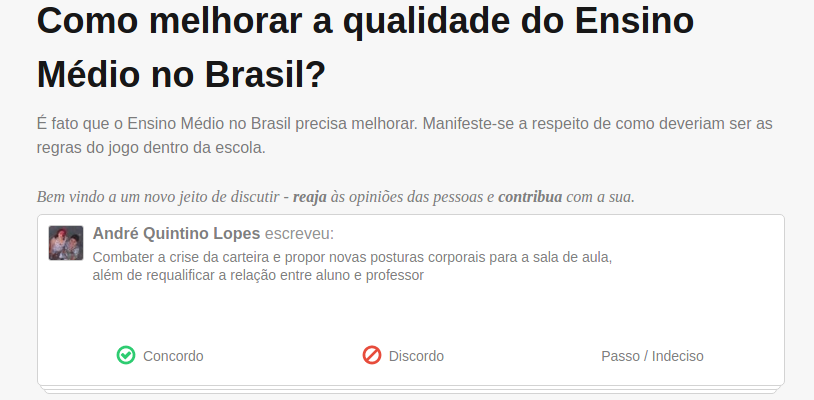
\includegraphics[width=.9\linewidth]{images/polis1.png}
     \caption{Cards with comments.}
     \label{fig:polis-1}
   \end{minipage}
   \begin{minipage}{.49\textwidth}
     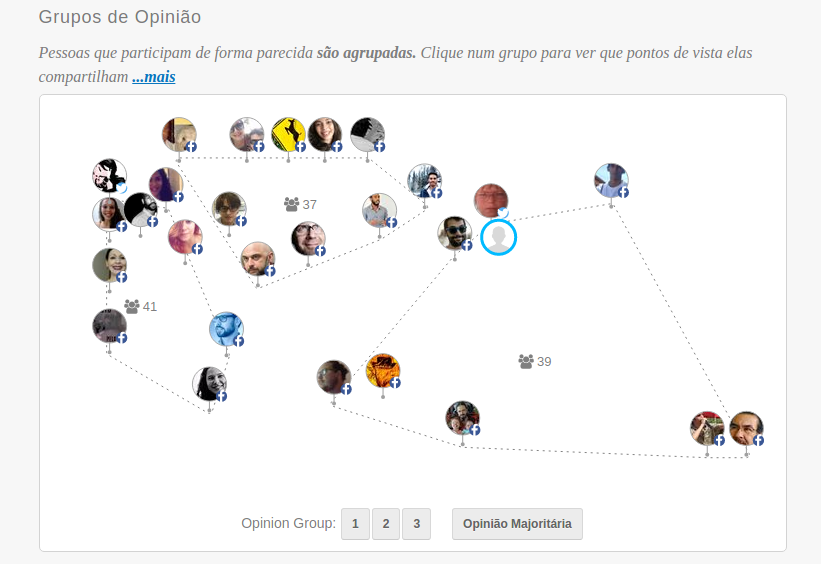
\includegraphics[width=.9\linewidth]{images/polis2.png}
     \caption{Groups of opinion formed.}
     \label{fig:polis-2}
   \end{minipage}
 \end{figure}

  The engagement of Polis CEO, Colin Megill, and one of its developer during the
two week laboratory period was important for us to understand how we could use
the Polis API on our project. At the beginning, Polis was licensed on an open
source BSD Licence and it was changed to
aGPLv3 \footnote{\url{https://www.gnu.org/licenses/gpl-3.0.en.html}}
Free Software licence along the hackathon! This change was very celebrated by
the Medialab Prado community.

  But despite Polis had became a free software, the code is miss documented and
very few people are able to understand it, beyond the company developers. Also,
Polis lacks features that we consider important for a participation tool, such
as resources to foment communication between people engaged in a duscussion. 
Those were some relevant obstacles to contribute to it and we had many 
difficulties through this approach. We understand that as a commercial company,
Polis is investing in forming an user community that can use and develop on top of what
is already working on Polis API. And they are very open to that. But they lack
a strategy to form a development community that can work on improvement of
Polis technology itself. Today they are not able to deal with external
contributions on code, even for people that want to deploy Polis on their
development environments. This can be acceptable within the short-term, but
will not be sustainable for the long-term.

\section{The Pushing Together project}
\label{sec:pushingtogether}

  Pushing Together project was born in a kind of a Hackathon. The project was
proposed by a Brazilian non-governmental organization called Cidade Democr\'atica
to the Collective Intelligence for Democracy Laboratory that was organized by
MediaLab Prado Madrid, Spain, in September/2016.

  With the goal of making the participation an easier process, fostering
engagement and breaking opinion bubbles, the project makes use of the
push notifications resource that we named ``the Push'', which is part of gamification
concept. Users in ownership of this ``power'' are able to send
messages and create events to engage participants inside the platform.

 Making an analysis about the users opinions, we initially identify three
 profiles based on their position on Polis dashboard, that are considered the potential
 receptors for ``the Push'' power with its derivative effects. With this
 initial profiles we intend to get a different interaction level between
 the multiple opinions groups of participative processes. However, this is still
 to be tested and validated for consolidation.

 \begin{figure}[hbt]
   \centering
     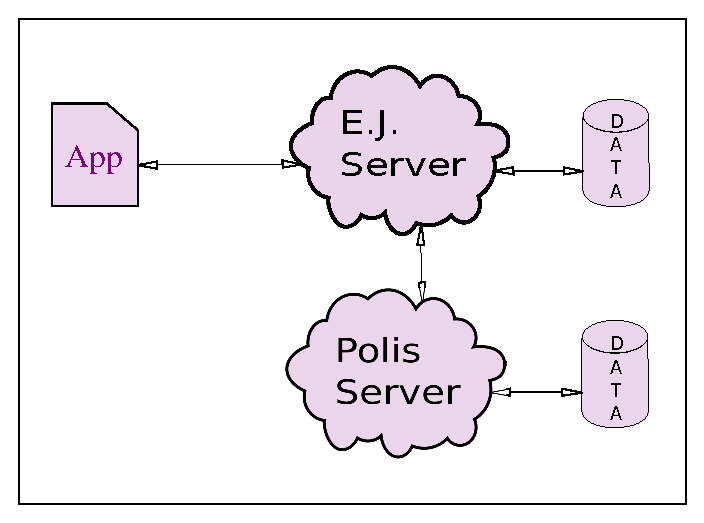
\includegraphics[keepaspectratio=true,,scale=0.5]{images/architecture-1.eps}
   \caption{Simplified architecture of the system}
   \label{fig:architecture-2}
 \end{figure}

  From the technical side, the project is divided in a front-end
application, written in React Native\footnote{\url{facebook.github.io/react-native}}
NodeJS\footnote{\url{nodejs.org/en}} server. The server module is responsible
for managing users, ``the Push'' resources for the gamification, and to make the
interface with the external cluster processing service, for which we reverse
engineered Polis.

\section{Final remarks}

  Pushing Together arise as a potential tool to bridge dialog between society
and the state, making different analyzes about the opinion of the distinct
groups and also opening new possibilities for the expression of these opinions
with ``the Push'' resource. Besides, the project was born with transparency and
collaboration principles, building a base for a prospective evolution.

  We are now working on a research to evolve the clustering service that will
fit our application model. Parallelly, our next steps include evolving the
mobile application using mocked data and validating the user interface.  All
our contributions are published in open repositories available at
\url{github.com/cidadedemocratica/pushingtogether} and
\url{github.com/cidadedemocratica/app\_pushingtogether}.

\bibliographystyle{plain}
\bibliography{references}

\end{document}
